\documentclass[border=12pt]{standalone}
\usepackage{tikz}
\usetikzlibrary{calc,intersections}

\begin{document}
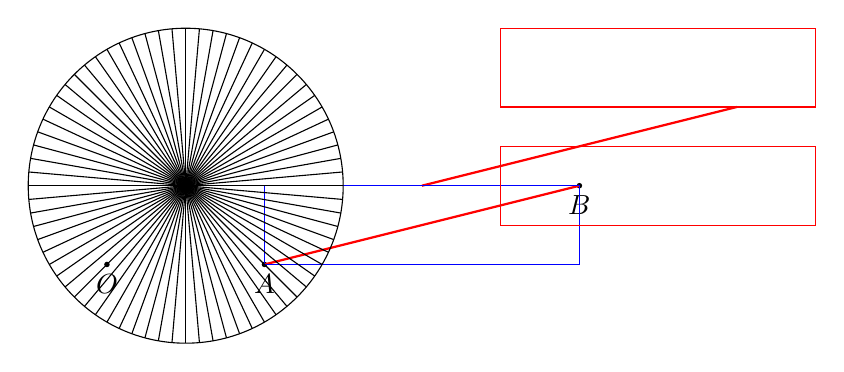
\begin{tikzpicture}
\coordinate (O) at (0,0);
\fill (O) circle(1pt) node [below] {$O$};
\coordinate (A) at (2,0);
\coordinate (B) at (6,1);
\coordinate (C) at (3,2);

\fill (A) circle(1pt) node [below] {$A$};
\fill (B) circle(1pt) node [below] {$B$};

% 原线段
\draw[red, thick] (A) -- (B);
% 平移
\draw[red, thick, transform canvas={shift={(2,1)}}] (A) -- (B);

\draw [blue](A) rectangle (B);
\draw [red] ($(A)+(C)$)  rectangle ($(B)+(C)$) ;
\draw [red] ($(A)+0.5*(B)$)  rectangle ($(B)+0.5*(B)$) ;

% 绕端点 (1,1) 旋转30度
\foreach \deg in {0,5,...,360} {
	\draw [rotate around={\deg:(1,1)}] (1,1) -- (3,1);
}
\draw (1,1) circle(2);

\end{tikzpicture}
\end{document}
